\section{MoDiGen Metamodell}
In diesem Abschnitt wird der Ansatz erkl\"art, indem die Architektur des Metamodells beschrieben und um ein Beispiel erg\"anzt wird.

\subsection{Architektur}
Die MoDiGen Metamodell-Architektur (Abbildung \ref{fig:MoDiGen-Metamodel}) wurde mit dem Fokus auf Allgemeingültigkeit und Erhalt der Einfachheit entworfen. Erstellte Modelle werden, einschließlich der Instanzen, in standard konformen JSON gespeichert. Dadurch bietet MoDiGen eine sprachunabhängige Modellierung, sowie ein erhöhtes Maß an Skalierbarkeit gegenüber ECore.

\begin{figure*}[h]
\centering
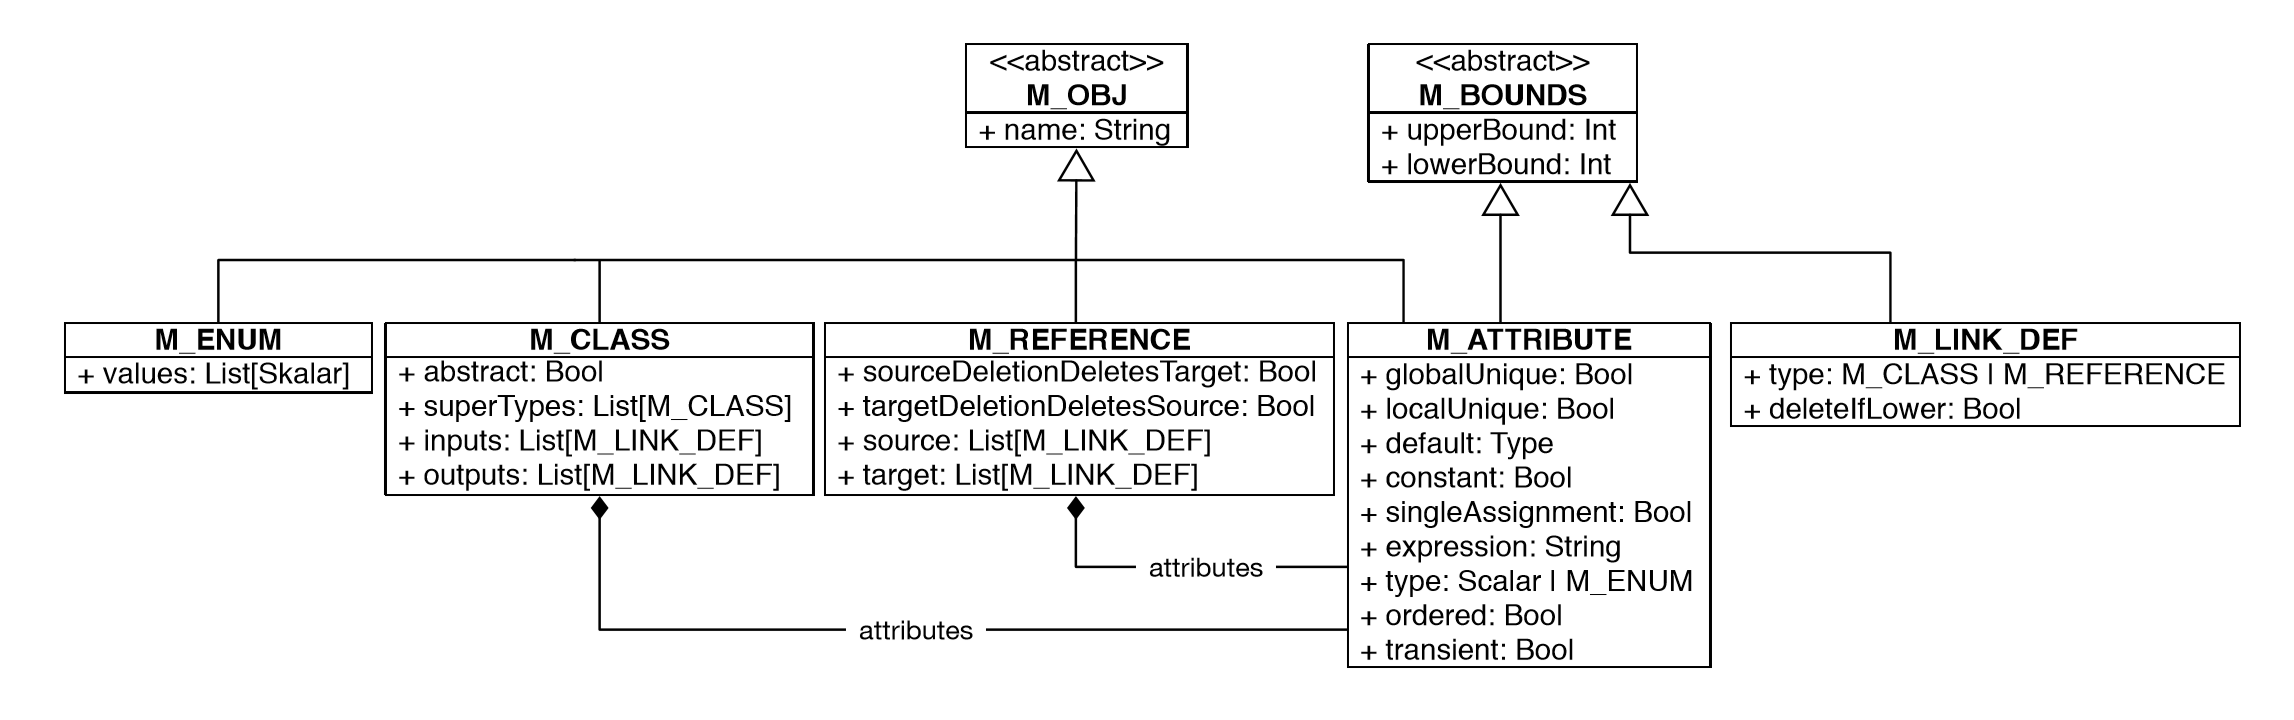
\includegraphics[width=\linewidth]{Abschnitte/Abbildungen/Grafiken/MoDiGen-Metamodel}
%
\epsfig{file=Quadrat.eps,height=1in,width=1in}
\caption{MoDiGen Metamodel}
\label{fig:MoDiGen-Metamodel}
\end{figure*}

Die abstrakte Klasse \texttt{M\_OBJ} enth\"alt das Attribut \textit{name}, dessen Wert innerhalb des gesamten Modells eindeutig ist. Dadurch wird es m\"oglich die erbenden Objekte zu identifizieren also die Instanzen von \texttt{M\_ENUM}, \texttt{M\_CLASS}, \texttt{M\_REFERENCE} und \texttt{M\_ATTRIBUTE}.
Eine Klasse mit ihren Attributen wird durch \texttt{M\_CLASS} und durch die Komposition zu \texttt{M\_ATTRIBUTE} im Modell erfasst. Vererbung wird durch das Attribut \textit{superTypes} modelliert. Hier ist anzumerken, dass auch Mehrfachvererbung dargestellt werden kann, da eine reflexive mehrfach Multiplizität vorliegt. 
Assoziationen werden durch \texttt{M\_LINK\_DEF} modelliert. Jede aus- bzw. eingehende Assoziation einer Klasse wird durch die Attribute \textit{inputs} und \textit{outputs} von \texttt{M\_CLASS} dargestellt, die auf \texttt{M\_LINK\_DEF} zeigen. Der \textit{typ} von \texttt{M\_LINK\_DEF} kann direkt eine \texttt{M\_CLASS} oder eine \texttt{M\_REFERENCE} sein. Durch \textit{deleteIfLower} wird bestimmt, ob die enthaltende \texttt{M\_CLASS} bzw. \texttt{M\_REFERENCE} zu löschen ist sobald \textit{lowerBound} unterschritten wird. Dies erm\"oglicht die modellierung von Kompositionen. Um beliebige Multiplizitäten und Rollen zu beschreiben, wird \texttt{M\_REFERENCE} verwendet. Dazu besitzt diese Klasse die Attribute \textit{source} und \textit{target}, die jeweils beliebig viele Instanzen von \texttt{M\_LINK\_DEF} referenzieren können. Die Attribute \textit{lower-} und \textit{upperBound} von \texttt{M\_LINK\_DEF} bestimmen die Multitplizität. Da \textit{source} und \textit{target} beliebig viele \texttt{M\_LINK\_DEF} referenzieren k\"onnen, lassen sich so n-\"are Assoziationen modellieren, die bei bedarf auch Assoziationen mit starker Bindung sein k\"onnen (Kompositionen).\\
Um Assoziationsklassen \cite{larman2005book}[S. 290] zu modellieren kann \texttt{M\_\-REF\-ER\-ENCE} beliebig viele Referenzen zu \texttt{M\_AT\-TRI\-BUTE} besitzen. \texttt{M\_ENUM} erg\"anzt das Metamodell um Aufz\"ahlungstypen, die \"uber \textit{type} von \texttt{M\_ATTRIBUTE} verwendet werden k\"onnen.\\
\texttt{M\_ATTRIBUTE} besitzt dahingehend noch weitere m\"oglichkeiten verschiedene Eigenschaften anzunehmen. \textit{globalUnique} besagt, dass der Wert des Attributes auf Modelebene unikat ist. \textit{localUnique} hingegen besagt, dass der Attributwert, sofern er Teil einer Collection ist, in diesem einmal sein muss. Um einen voreingestellten Wert zu bestimmen wird das Attribut \textit{default} verwendet. Ist bspw. \textit{constant} auf true gesetzt, so wird default als endg\"ultiger Wert angenommen. Eine andere m\"oglichkeit bietet \textit{singleAssignment}. Ist dessen Wert true, so lässt sich dem Attribut nur einmal ein Wert zuordnen. \textit{type} bestimmt entweder einen generischen Typ (hier \texttt{Skalar} genannt) oder einen Aufz\"ahlungstypen \texttt{M\_ENUM}. \textit{expression} erm\"oglicht es eine Formel zu bestimmen, die den Wert des Attributes berechnet. Mit \textit{ordered} kann festgelegt werden dass die Werte des Attributes sortiert sind. Es ist dabei nicht angegeben in welcher Art und Weise sortiert ist. Um einfluss auf die Speicherung des Attributes zu nehmen kann \textit{transient} verwendet werden. Ist es auf true gesetzt, so werden die Werte dieses Attributs nicht persistiert. 


\subsection{Beispiel}
Um das zugrundeliegende JSON-Format n\"aher zu beschreiben, wird im Folgenden als Beispiel ein vereinfachter Familienstammbaum verwendet (siehe Abbildung \ref{fig:Family-Tree-Model}).\\ 
Es existiert eine Entiät \texttt{Person}, die \textit{Vornamen}, \textit{Sozialversicherungsnummer} und \textit{Geburtstag} als Attribute besitzt. Die beiden Klassen \texttt{Male} und \texttt{Female} erben von \texttt{Person} und besitzen keine Attribute. Dabei kann \texttt{Male} eine Assoziation zu \texttt{Female} mit der Rolle \textit{isHusband} haben und, umgekehrt, die Klasse \texttt{Female} zu \texttt{Male} mit der Rolle \textit{isWife}. Das Eltern-Kind verh\"altnis wird durch 1-zu-m Assoziationen von \texttt{Female} bzw. \texttt{Male} zu \texttt{Person} und der dazugeh\"origen Rolle (\textit{isMother}, \textit{isFather}) beschrieben.

\begin{figure}[H]
\centering
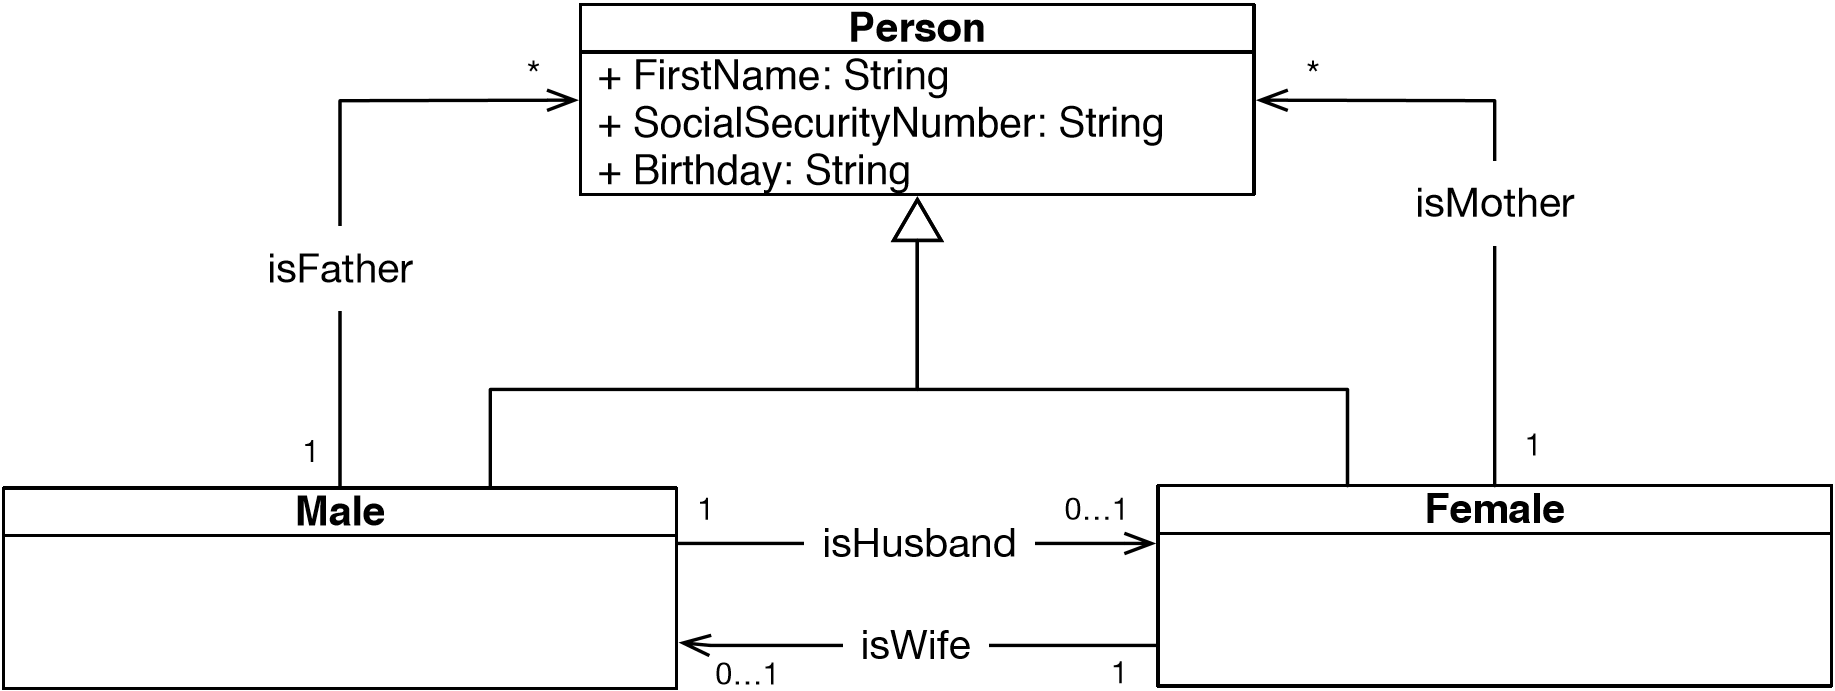
\includegraphics[width=\linewidth]{Abschnitte/Abbildungen/Grafiken/Family-Tree-Model}
\caption{Family Tree Model}
\label{fig:Family-Tree-Model}
\end{figure}


Die Klasse \texttt{Male} kann wie Listing \ref{lst:malejson} zeigt als JSON gespeichert werden. Dabei wird das JSON-Objekt \"uber den Klassennamen identifiziert -- hier \textit{Male} -- und durch das Attribut \textit{mType} als Klasse bestimmt. Da JSON keine implizite Typisierung unterstützt -- es unterscheidet lediglich zwischen wenigen generischen Datentypen -- muss hier explizit festgelegt werden, dass es sich um \textit{mClass} handelt. Die Assoziationen werden entsprechend als JSON-Arrays \textit{inputs} und \textit{outputs} gespeichert und enthalten die durch \texttt{M\_LINK\_DEF} definierten Attribute.

\lstlistingCode{M\_CLASS Male aus dem Family Tree Beispiel}{malejson}
"Male": { 
  "mType": "mClass", 
  "name": "Male",
  "superTypes": ["Person"], 
  "mAttributes": [], 
  "inputs": [{ 
    "type": "isWife", 
    "upperBound": 1, 
    "lowerBound": 0 
  }], 
  "outputs": [{ 
    "type": "isHusband", 
    "upperBound": 1,
    "lowerBound": 0 
    },{ 
    "type": "isFather", 
    "upperBound": -1,
    "lowerBound": 0
  }] 
}
\end{lstlisting}

Eine \texttt{M\_REFERENCE} wird als "`Objekt erster Klasse"' gespeichert wie Listing \ref{lst:ishusbandjson} zeigt und kann damit unabhängig von den \texttt{M\_CLASS} instanzen geladen werden. Das JSON-Objekt wird durch den Namen der \texttt{M\_REFERENCE} identifiziert und enth\"alt alle Attribute. Der Typ wird hier, wie bei \texttt{M\_CLASS} instanzen in \textit{mType} abgelegt. In den JSON-Arrays \textit{source} und \textit{target} werden, genau wie bei den \texttt{M\_CLASS} instanzen, die gesamten \texttt{M\_LINK\_DEF} instanzen abgelegt. In diesem Modell kann \texttt{Male} eine Assoziation der Rolle \textit{isHusband} haben. Diese \texttt{M\_LINK\_DEF} instanz zeigt auf die entsprechende \texttt{M\_REFERENCE} instanz, die wiederrum mit zwei Endpunkten zu \texttt{Female} und \texttt{Male} existiert. Im hinblick auf \textit{upper-/lowerBounds}, die jeweils eins sind, wird der Sachverhalt "`Ein Ehemann ist der Mann einer Frau"' modelliert.

\lstlistingCode{Husband M\_REFERENCE Male aus dem Family Tree Beispiel}{ishusbandjson}
"isHusband": {
  "mType": "mRef", 
  "name": "isHusband",
  "mAttributes": [], 
  "source": [{ 
    "type": "Male", 
    "upperBound": 1, 
    "lowerBound": 1 
  }], 
  "target": [{ 
    "type": "Female", 
    "upperBound": 1, 
    "lowerBound": 1, 
  }] 
} 
\end{lstlisting}

Die Instanzen werden durch UUIDs identifiziert und enthalten Verweise auf ihre Typen im Modell sowie ihre Typen im Metamodell. Dies ist z.B durch die Kombination \textit{"`mClass"': "`Male"'} in Zeile 2 von Listing \ref{lst:instancejson} zu sehen. Es handelt sich um eine Instanz von \texttt{Male}, die wiederrum als Klasse, also als Instanz von \texttt{M\_CLASS} modelliert ist. Die \textit{outputs} und \textit{inputs} verweisen hier auf Instanzen von konkreten Referenzen -- in diesem Fall \textit{isHusband}, \textit{isWife} und \textit{isFather}.\\
Die Referenz \textit{isHusband} zeigt gemäß des Modells (Abbildung \ref{fig:Family-Tree-Model}) in \textit{source} auf eine Instanz von \texttt{Male} und in \textit{target} auf eine Instanz von \texttt{female}.

\lstlistingCode{Family Tree Instanz}{instancejson}
"846bc8a2-00fc-401f-b626-0b0252516aee": { 
  "mClass": "Male", 
  "outputs": { 
    "isFather": 
      ["8e9b1093-a589-4ae4-8e1e-1b3d63a3f842"], 
    "isHusband": 
      ["ee204744-6322-49d4-928e-1442e8bc70c4"] 
  }, 
  "inputs": { 
    "isWife": 
      ["666d4de7-e0f2-4620-8c19-d5469b40be1f"] 
  }, 
  "mAttributes": { 
    "First_Name": ["Hans"], 
    "SocialSecurityNumber": ["12"], 
    "Birthday": ["12-02-2015"] 
  } 
}, 

"ee204744-6322-49d4-928e-1442e8bc70c4": { 
  "mRef": "isHusband", 
  "source": { 
    "Male": 
      ["846bc8a2-00fc-401f-b626-0b0252516aee"] 
  }, 
  "target": { 
    "Female": 
      ["a264a43b-6f97-4257-9243-baddbf745490"] 
  } 
} 
\end{lstlisting}
